\section{Communication-Efficient Model Parallelism}\label{sect:method}
\vspace{-4pt}

In this section, we outline our approach for training large models with heterogeneous unreliable poorly-connected devices.
To that end, the section is organized as follows:

\vspace{-4pt}
\begin{itemize}
    \item Section~\ref{sect:method_squarecube} analyzes how existing model-parallel algorithms scale with model size and shows conditions where training increasingly larger models leads to less intense network usage;
    \item Section~\ref{sect:method_swarm} describes SWARM parallelism --- a decentralized algorithm for training large models under the conditions outlined in Section~\ref{sect:related_cost_efficent_collaborative}.
\end{itemize}
\vspace{-12pt}

\subsection{The Square-Cube Law of Distributed Training}\label{sect:method_squarecube}

To better understand the general scaling properties of model parallelism, we need to abstract away from the application-specific parameters, such as model architecture, batch size, and system design. To that end, we first consider a simplified model of pipeline parallelism. Our ``pipeline'' consists of $k$ stages, each represented by $n{\times}n$ matrices. Intuitively, the first matrix represents the input data and all subsequent matrices are linear ``layers'' applied to that data. This model abstracts away from application-specific details, allowing us to capture general relationships that hold for many models.

During ``training'', stages iteratively perform matrix multiplication and then send the output to the subsequent pipeline stage over a throughput-limited network. These two operations have different scaling properties.
The compute time for naïve matrix multiplication scales as $O(n^3)$. While this can be reduced further in theory~\citep{coppersmith_winograd,refined_laser}, it is only used for very large matrices~\citep{practical_matmul_best,practical_matmul_earlier,strassen_reloaded}. Therefore, deep learning on GPUs typically relies on $O(n^3)$ algorithms.


In turn, the communication phase requires at most $O(n^2)$ time to transfer a batch of $n{\times}n$ activations or gradients. Therefore, as we increase the model size, the computation time grows faster than communication time, regardless of which matrix multiplication algorithm we use. We refer to this idea as the \textit{square-cube law} after the eponymous principle in physics~\citep{square_cube,mechanics}.

This principle applies to many real-world neural network architectures, albeit with some confounding variables. In convolutional neural networks~\cite{conv_first}, the computation time scales as $O(B H W C^2)$ and the communication is $O(B H W C)$, where $B$, $H$, $W$ and $C$ stand for batch size, height, width and the number of channels. Recurrent neural networks~\citep{backprop_rnn,lstm} need $O(B L H^2)$ compute in terms of batch size, sequence length, and hidden size, respectively, and $O(B L H)$ or $O(B H)$ communication, depending on the architecture. With the same notation, Transformers~\citep{transformer} require $O(B L^2 H)$ compute for attention layers, $O(B L H^2)$ compute for feedforward layers, but only $O(B L H)$ communication.%


Based on these observations, we conclude that pipeline parallelism naturally grows more communication-efficient with model size. More precisely, increasing the hidden dimension will reduce the communication load per device per unit of time, making it possible to train the model efficiently \textit{with lower network bandwidth} and \textit{higher latency}\footnote{Latency slows the communication down by a constant factor that also grows less important with model size.}. While the exact practical ramifications depend on the use case, Section~\ref{sect:experiments_square_cube} demonstrates that some of the larger models trained with pipeline parallelism can already train at peak efficiency with only hundreds of Mb/s bandwidth.


In theory, the square-cube principle also applies to intra-layer parallelism, but using this technique at 500 Mb/s would become practical only for layer sizes of more than $2^{16}$ units. Data-parallel training with sharding or offloading~\citep{zerooffload} does not scale as well, as its communication time scales with the size of \textit{model parameters} instead of activations. However, it may be possible to achieve similar scaling with gradient compression algorithms.


\subsection{SWARM Parallelism}\label{sect:method_swarm}

Traditional pipeline parallelism can be communication-efficient, but this alone is not enough for our setups. Since training devices can have different compute and network capabilities, a pipeline formed out of such devices would be bottlenecked by the single ``weakest link'', i.e., the participant with the smallest training throughput. As a result, the more powerful nodes along the pipeline would be underutilized due to either lack of inputs or slow subsequent stages. On top of that, if any node fails or leaves training prematurely, it will stall the entire training procedure.

\begin{figure*}[t]
    \centering
    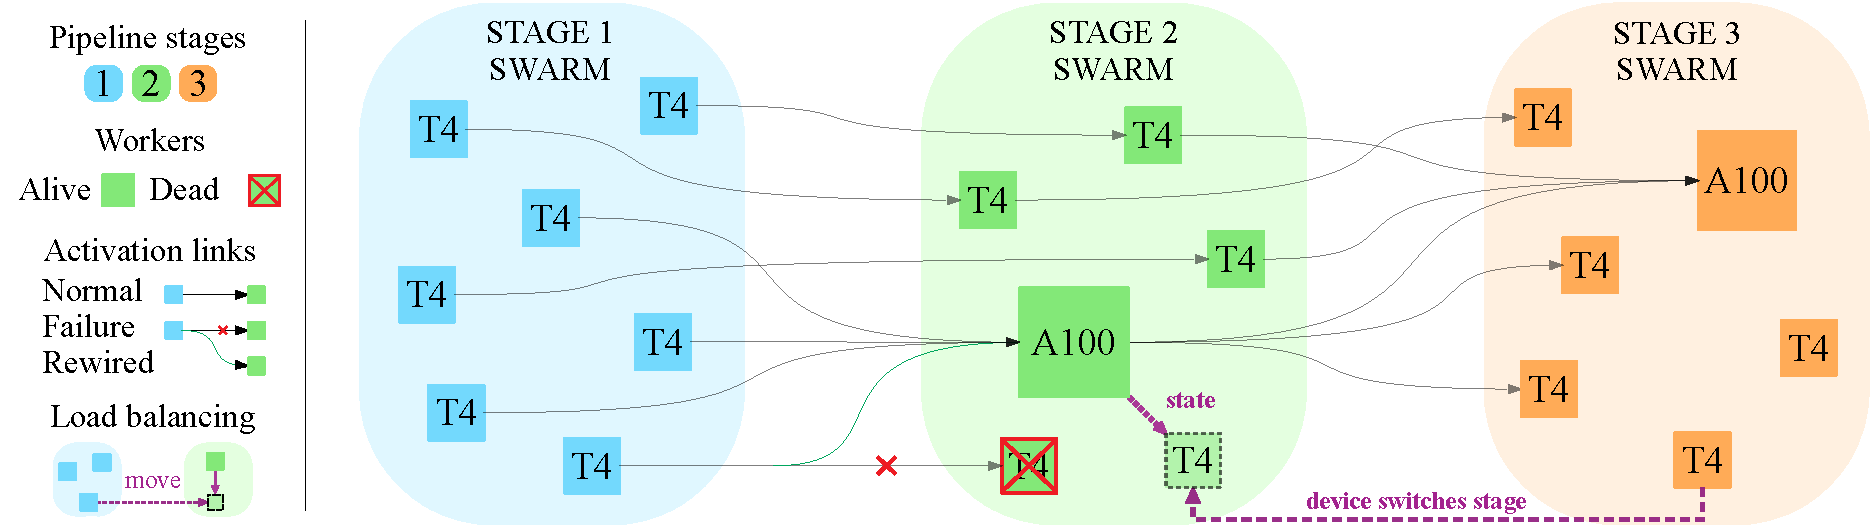
\includegraphics[width=\linewidth]{resources/swarm_v2_max.pdf}
    \caption{An overview of SWARM parallelism, illustrating both normal operation, device failures and adaptive rebalancing. One of the workers at stage 2 leaves; another peer from stage 3 takes its place by downloading the latest stage 2 parameters and statistics from peers.}
    \label{fig:swarm}
    \vspace{-12pt}
\end{figure*}

To overcome these two challenges, we replace the rigid pipeline structure with temporary ``pipelines'' that are built stochastically on the fly during each iteration. Each participant can send their outputs to any peer that serves the next pipeline stage. Thus, if one peer is faster than others, it can process inputs from multiple predecessors and distribute its outputs across several weaker peers to maximize utilization. Also, if any participant disconnects, its predecessors can reroute their requests to its neighbors. New peers can download up-to-date parameters and optimizer statistics from remaining workers at the chosen stage. This allows the training to proceed as long as there is at least one active participant per stage: we elaborate on the fault tolerance of SWARM parallelism in Appendix~\ref{appendix:faq}.

The resulting system consists of several consecutive swarms, as depicted in Figure~\ref{fig:swarm}. Peers within one swarm serve the same pipeline stage (i.e., the \textbf{same subset of layers} with \textbf{the same parameters}).
We assume that the model consists of similar ``blocks'' and thus partition it into evenly sized stages, leaving the study of better strategies~\citep{huang2019gpipe,pipedream} as future work.
During the \textit{forward} pass, peers receive inputs from predecessors (determined on each iteration) and send activations to peers in the next stage. For the \textit{backward} pass, peers receive gradients for outputs, compute gradients for layer inputs and accumulate gradients for parameters. Once enough gradients are accumulated, peers form groups, run All-Reduce to average gradients within their pipeline stages and perform the optimizer step.

SWARM parallelism can also use Delayed Parameter Updates~(DPU)~\citep{zerooffload} to further improve hardware utilization by performing the optimizer step in parallel with processing the next batch. While it is technically asynchronous, DPU was shown to achieve similar per-iteration convergence as fully synchronous training, both theoretically~\citep{stich2020error,arjevani2020tight} and empirically~\citep{zerooffload,dedloc}.

Each peer has queues for incoming and outgoing requests to maintain high GPU utilization under latency and to compensate for varying network speeds. Similarly to other pipeline implementations~\citep{huang2019gpipe,megatron2}, SWARM parallelism uses activation checkpointing~\citep{gradient_checkpointing_autograd, gradient_checkpointing_dl} to reduce the memory footprint. %


\vspace{-6pt}
\paragraph{Stochastic wiring.} To better utilize heterogeneous devices and recover from faults, we dynamically ``wire'' each input through each stage and pick devices in proportion to their training throughput. To achieve this, SWARM peers run ``trainer'' processes that route training data through the ``stages'' of SWARM, balancing the load between peers.

For each pipeline stage, trainers discover which peers currently serve this stage via a Distributed Hash Table (DHT,~\citealp{kademlia}). Trainers then assign a microbatch to one of those peers based on their performance. If that peer fails, it is temporarily banned and the microbatch is sent to another peer within the same stage. Note that trainers themselves do not use GPUs and have no trainable parameters, which makes it possible to run multiple trainers per peer. 

Each trainer assigns data independently using the Interleaved Weighted Round-Robin~\citep{iwrr,interleaved_round_robin} scheduler. Our specific implementation of IWRR uses a priority queue: each peer is associated with \textit{the total processing time over all previous requests}. A training minibatch is then routed to the node that has the smallest total processing time. Thus, for instance, if device A takes half as long to process a sample as device B, the routing algorithm will choose A twice as often as B. Finally, if a peer does not respond or fails to process the batch, trainer will ``ban'' this peer until it reannounces itself in the DHT, which is done every few minutes. For a more detailed description of stochastic wiring, please refer to Appendix~\ref{appendix:wiring_details}.

Curiously, different trainers can have different throughput estimates for the same device because of the network topology. For instance, if training nodes are split between two cloud regions, a given peer's trainer will have a higher throughput estimate for peers in the same data center. In other words, trainers automatically adjust to the network topology by routing more traffic to peers that are ``nearby''.

\vspace{-8pt}
\paragraph{Adaptive swarm rebalancing.} While stochastic wiring allows for automatic rebalancing within a stage, additional cross-stage rebalancing may be required to maximize throughput, especially when devices are very unreliable. As we described in Section~\ref{sect:related_cost_efficent_collaborative}, our workers can join and leave training at any time. If any single pipeline stage loses too many peers, the remaining ones will face an increased processing load, which will inevitably form a bottleneck. 

SWARM parallelism addresses this problem by allowing peers to dynamically switch between ``pipeline stages'' to maximize the training throughput. Every $T$ seconds, peers measure the utilization rate of each pipeline stage as the queue size.
Peers from the most underutilized pipeline stage will then switch to the most overutilized one (see Figure~\ref{fig:swarm} for an overview and Appendix~\ref{appendix:rebalancing_formal} for a formal description and complexity analysis), download the latest training state from their new neighbors and continue training. Similarly, if a new peer joins midway through training, it is assigned to the optimal pipeline stage by following the same protocol. As a side effect, if one pipeline stage requires more compute than others, SWARM will allocate more peers to that stage. In Section~\ref{sect:experiments_adaptive}, we evaluate our approach to dynamic rebalancing in realistic conditions.









